\documentclass[twoside,11pt]{article}

% Any additional packages needed should be included after jmlr2e.
% Note that jmlr2e.sty includes epsfig, amssymb, natbib and graphicx,
% and defines many common macros, such as 'proof' and 'example'.
%
% It also sets the bibliographystyle to plainnat; for more information on
% natbib citation styles, see the natbib documentation, a copy of which
% is archived at http://www.jmlr.org/format/natbib.pdf

\usepackage{jmlr2e}
\usepackage{amsmath}
\usepackage[utf8]{inputenc} % allow utf-8 input
\usepackage[T1]{fontenc}    % use 8-bit T1 fonts
%\usepackage{hyperref}       % hyperlinks
\usepackage{url}            % simple URL typesetting
\usepackage{booktabs}       % professional-quality tables
\usepackage{amsfonts}       % blackboard math symbols
\usepackage{nicefrac}       % compact symbols for 1/2, etc.
\usepackage{microtype}      % microtypography
\usepackage{mathrsfs}
\usepackage{amssymb}
\usepackage{subfigure}
\usepackage{algorithm}  
\usepackage{algorithmic}  
\usepackage{graphicx}


\renewcommand{\algorithmicrequire}{\textbf{Input:}}
\renewcommand{\algorithmicensure}{\textbf{Output:}}


% Definitions of handy macros can go here


%\newtheorem{theorem}{Theorem} 
%\newtheorem{remark}{Remark} 
%\newtheorem{corollary}{Corollary} 
%\newtheorem{lemma}{Lemma}[subsection]
%\newtheorem{proposition}{Proposition} 
\newtheorem{assumption}{Assumption}
%\newtheorem{definition}{Definition} 
\numberwithin{equation}{section}

\newcommand{\dataset}{{\cal D}}
\newcommand{\fracpartial}[2]{\frac{\partial #1}{\partial  #2}}

\newcommand{\E}{\mathbb{E}}
\newcommand{\p}[2]{\mathbb{P}_{[#1]}^{#2}}
\newcommand{\pp}[2]{p_{[#1]}^{#2}}
\newcommand{\huaf}{\mathcal{F}}
\newcommand\numberthis{\addtocounter{equation}{1}\tag{\theequation}}

\graphicspath{{../figure/}}


% Heading arguments are {volume}{year}{pages}{submitted}{published}{author-full-names}

\jmlrheading{1}{2000}{1-48}{4/00}{10/00}{meila00a}{Marina Meil\u{a} and Michael I. Jordan}

% Short headings should be running head and authors last names

\ShortHeadings{Learning with Mixtures of Trees}{Meil\u{a} and Jordan}
\firstpageno{1}

\begin{document}

\title{Finite sample analysis of the GTD Policy Evaluation Algorithms in Markov Setting}

%\author{\name Marina Meil\u{a} \email mmp@stat.washington.edu \\
%       \addr Department of Statistics\\
%       University of Washington\\
%       Seattle, WA 98195-4322, USA
%       \AND
%       \name Michael I.\ Jordan \email jordan@cs.berkeley.edu \\
%       \addr Division of Computer Science and Department of Statistics\\
%       University of California\\
%       Berkeley, CA 94720-1776, USA}
\author{Yue Wang}

\editor{Kevin Murphy and Bernhard Sch{\"o}lkopf}

\maketitle

\begin{abstract}%   <- trailing '%' for backward compatibility of .sty file
		In reinforcement learning (RL), the key component is policy evaluation, which aims to estimate the value function (i.e., expected long-term accumulated reward starting from a state) of a given policy. With a good policy evaluation method, the RL algorithms can estimate the value functions of the given policy more accurately and find a better policy. When the state space is large or continuous, \emph{Gradient-based Temporal Difference(GTD)} algorithms with linear function approximation to the value function are widely used. Considering that the collection of the evaluation data is very likely to be both time and reward consuming, to get a clear understanding of the finite sample performance of the GTD algorithms is very important to the efficiency of policy evaluation and the entire RL algorithms. Previous work converted GTD algorithms into a convex-concave saddle point problem and provided the finite sample analysis of the GTD algorithms with constant step size  under the assumption that data are i.i.d. generated. However, as we know, in RL problems, the data are generated from Markov processes rather than i.i.d. and step size  is set in different ways. In this paper, in the realistic Markov setting, we derive finite sample bounds both in expectation and with high probability for the general convex-concave saddle point problem, and hence for the GTD algorithms. Our bounds show that, in the Markov  setting, (1) with variants of step size, GTD algorithms converge; (2) the convergence rate is determined by the step size, and related to the mixing time of the Markov process; (3) we explain that the experience reply trick is effective, since it can improve the mixing property of the Markov process.  To the best of our knowledge, our analysis is the first to provide finite sample bounds for the GTD algorithms in Markov setting. 

\end{abstract}

\begin{keywords}
  Bayesian Networks, Mixture Models, Chow-Liu Trees
\end{keywords}

\section{Introduction}

	Reinforcement Learning (RL) (\cite{sutton1998reinforcement}) technologies are very powerful to learn how to interact with environments, and has variants of important applications, such as robotics, computer games and so on (\cite{kober2013reinforcement}, \cite{mnih2015human}, \cite{silver2016mastering}, \cite{bahdanau2016actor}). 
	
	In RL problem, an agent observes the current state, takes an action following a policy based on the current state, receives a reward from the environment, and the environment transits to the next state in Markov, and again repeats these steps. The goal of  the RL algorithms is to find the optimal policy which leads to the maximum long-term reward. The value function of a fixed policy for a   state is defined as the expected long-term accumulated reward the agent would receive by following the fixed policy starting from this state. Policy evaluation aims to accurately estimate the value of all states under a given policy, which is a key component in RL (\cite{sutton1998reinforcement}, \cite{dann2014policy}). A better policy evaluation method will help us to improve the current policy and find the optimal policy.
	
	When the state space is large or continuous, it is inefficient to represent the value function over all the states by a look-up table. A common approach is to extract features for states and use parameterized function over the feature space to approximate the value function. In applications, there are linear approximation and non-linear approximation (e.g. neural networks) to the value function. In this paper, we will focus on the linear approximation (\cite{sutton2009convergent},\cite{sutton2009fast},\cite{liu2015finite}). Leveraging the localization technique in \cite{bhatnagar2009convergent}, the results can be generated into non-linear cases with extra efforts. We leave it as future work. 
	
	In policy evaluation with linear approximation, there were substantial work on the temporal-difference (TD) method, which uses the Bellman equation to update the value function during the learning process (\cite{sutton1988learning},\cite{tsitsiklis1997analysis}). Recently, \cite{sutton2009convergent} \cite{sutton2009fast} have proposed \emph{Gradient-based Temporal Difference (GTD)} algorithms which use gradient information of the error from the Bellman equation to update the value function.  It is shown that, GTD algorithms have achieved the lower-bound of the storage and computation complexity, making them powerful to handle high dimensional big data.  Therefore, now GTD algorithms are widely used in policy evaluation problem and the policy evaluation step in practical RL algorithms (\cite{bhatnagar2009convergent},\cite{silver2014deterministic}).  %, and researchers are keep improving GTD algorithms by designing different step size  and empirical tricks like experience reply \cite{}\cite{}.
	
	
	However, we don’t have sufficient theory to tell us about the finite sample performance of the GTD algorithms. To be specific, will the evaluation process converge? If yes, how many samples we need to get a target evaluation error? Will the step size in GTD algorithms influence the finite sample error? How to explain the effectiveness of the practical tricks, such as experience reply? Considering that the collection of the evaluation data is very likely to be both time and reward consuming, to get a clear understanding of the finite sample performance of the GTD algorithms is very important to the efficiency of policy evaluation and the entire RL algorithms.
	
	Previous work (\cite{liu2015finite}) converted the objective function of GTD algorithms into a convex-concave saddle problem and conduct the finite sample analysis for GTD with constant step size in the independent and identical distributed (i.i.d.) setting in which data are simply assumed to be generated by  i.i.d.. However, in RL problem, the date are generated from an agent who interacts with the environment step by step, and the state will transit in Markov as introduced previously. As a result, the data are generated from a Markov process but not i.i.d..  In addition, the work did not study the decreasing step size , which are also commonly-used  in many gradient based algorithms(\cite{sutton2009convergent},\cite{sutton2009fast},\cite{yu2015convergence}). Thus, the results from previous work cannot provide precise answers to the above questions for the finite sample performance of the GTD algorithms.
	
	In this paper, we perform the finite sample analysis for the GTD algorithms in the more realistic Markov setting. To achieve the goal, first of all, same with \cite{liu2015finite}, we consider the stochastic gradient descent algorithms of the general convex-concave saddle point problems, which include the GTD algorithms. The quality of the solution is measured by the primal-dual gap in the convex-concave saddle point optimization problem (\cite{liu2015finite} , \cite{nemirovski2009robust}).	
	The   finite sample analysis for convex-concave optimization in Markov setting is challenging. On one hand, in Markov setting, the non-i.i.d. sampled gradients are no longer unbiased estimation of the gradients. Thus, the proof technique for i.i.d. setting cannot be applied. On the other hand, although for convex optimization problem, with the Markov gradients, SGD still has convergence guarantee, it is much more difficult to obtain the same results in the more complex convex-concave optimization problem.  
	
	
	To overcome the challenge, we design a novel decomposition ( ) of the error function. The intuition of the decomposition and key techniques are as follows:  {(1)} Although samples are not i.i.d., for large enough $ \tau $, the sample at time $t+\tau$ is "nearly independent"  of the sample  at time $t$, and its distribution is "very close" to the stationary distribution.  {(2)} We split the random variables in the objective related to $ \mathbf{\E} $ operator and the variables related to $ \mathbf{\max} $ operator into different terms in order to control them respectively. It is non-trivial, and we construct a sequence of auxiliary random variables to do so.  {(3)} All constructions above need to be carefully considered the measurable issues in the Markov setting. 
	
	By using the above techniques, we prove a novel finite sample bound in expectation for the convex-concave saddle point problem. Based on the bound in expectation, we construct martingale difference sequences and apply Azuma's inequality to obtain the finite sample bound with high probability. Considering the GTD algorithms are specific convex-concave saddle point optimization methods, we finally obtained the finite sample bounds in expectation and with high probability for the GTD algorithms, in the realistic Markov setting for RL. To the best of our knowledge, our analysis is the first to provide finite sample bounds for the GTD algorithms in Markov setting.
	
	We have the following discussions based on our finite sample bounds. \\
	(1) GTD algorithms do converge, under a flexible condition on the step size, i.e.  $\sum_{t=1}^{T}\alpha_t \to \infty, \frac{\sum_{t=1}^{T}\alpha_t^2}{\sum_{t=1}^{T}\alpha_t} <\infty $, as $T\to \infty$, where $\alpha_t$ is the step size. The popular step size  settings all satisfy this condition. \\
	(2) The convergence rate in expectation is     $ \mathcal{O}\left(\sqrt{(1+\tau(\eta))\frac{\sum_{t=1}^{T}\alpha_t^2}{\sum_{t=1}^{T}\alpha_t }}  \right) $  and with   probability $ 1-\delta $ is    $ \mathcal{O}\left(\sqrt{(1+\tau(\eta))\frac{\sum_{t=1}^{T}\alpha_t^2}{\sum_{t=1}^{T}\alpha_t } + \frac{\sqrt{\tau(\eta)\log(\frac{\tau(\eta)}{\delta}) \sum_{t=1}^{T}\alpha_t^2}} {\sum_{t=1}^{T}\alpha_t}}  \right)  $ , where $\tau(\eta)$   is the mixing time of the Markov process, and $\eta$ is a constant. Different step size  will lead to different convergence rates.\\
	(3) The experience reply trick is effective, since it can improve the mixing property of the Markov process.  
	
	Finally, we conduct simulation experiments to verify our theoretical founding. All the conclusions from the analysis are consistent with our empirical observations. 
	
 

\section{Background and Notation}


	In this section, we briefly introduce the GTD algorithms and related works.
	\subsection{Gradient-based TD algorithms}
		Consider the reinforcement learning problem with Markov decision process(MDP) $ (\mathcal{S},\mathcal{A},P,R,\gamma) $, where $ \mathcal{S} $ is the state space, $ \mathcal{A} $ is the action space, $ P= \{P_{s,s'}^a; s,s’\in \mathcal{S}, a\in\mathcal{A}\} $ is the transition matrix and $ P_{s,s'}^a $ is the transition probability from state $ s $ to state $ s' $ after taking action $ a $, $ R=\{R(s,a );s\in \mathcal{S},a\in\mathcal{A}$ is the reward function and $R(s,a)$ is the reward received at state $s$ if taking action $a$, and $ 0<\gamma<1 $ is the discount factor. 	
		A policy function $ \mu : \mathcal{A}\times\mathcal{S}\to [0,1]$ indicates the probability to take each action at each state.  Value function for policy $ \mu $ is defined as: $ 	V^{\mu}(s)\triangleq E\left[ \sum_{t=0}^{\infty}\gamma^t R(s_t,a_t)|s_0 = s,\mu  \right] $.
		%	 	$$  . $$ 
		%Intuitively, the value function measure the expected long-term accumulated reward if we keep taking actions according to policy $\mu$, starting from state $s$. The goal of RL is to find the optimal policy with the maximum value.  The policy evaluation tasks aim to estimate the value of a policy by the data generated by interacting with the environment with this policy. i.e., $ \mathcal{D} = \left \lbrace \xi_i= (s_i,a_i,r_i,s_i') \right\rbrace_{i=1}^T $, where $ \xi_i $ are sampled from the Markov chain with transition probability $ p_{\xi_i,\xi_j} = \mu(s_i',a_j)P_{s,s'}^a(s_j'|s_j,a_j) $.	
		
		
		In order to perform policy evaluation in a large state space, states are represented by a feature vector $\phi(s)\in\mathbb{R}^d$, and a linear   function  $ \hat{v}(s) = \phi(s)^\top \theta  $
		is used to approximate the value function. The evaluation error is defined as  $ \Vert V(s) - \hat{v}(s) \Vert_{s\sim \pi} $, and $ \pi $ is a distribution over the state space $ \mathcal{S} $. The evaluation error can be decomposed into approximation error and estimation error. In this paper, we will focus on the estimation error with linear function approximation. 
		
		As we know, the value function in RL satisfies the following Bellman equation: $ V^\mu(s)   = \E_{\mu,P}\left[R(s_t,a_t)+\gamma V^\mu(s_{t+1}) | s_t=s \right] \triangleq T^\mu V^\mu(s)  $,
		where $ T^\mu  $ is called Bellman operator for policy $\mu$.
		Gradient-based TD (GTD) algorithms (including GTD and GTD2) proposed by \cite{sutton2009convergent} and \cite{sutton2009fast}  update the approximated value function by minimizing the objective function related to  Bellman equation errors, i.e., the  norm of the expected TD update (NEU) and mean-square projected Bellman error  (MSPBE) respectively(\cite{maei2011gradient},\cite{liu2015finite})	,
		\begin{align}
		GTD&:  \quad J_{NEU}(\theta)  =\Vert \Phi^\top K (T^\mu\hat{v}-\hat{v}) \Vert^2\\
		GTD2&: \quad J_{MSPBE}(\theta)  = \Vert \hat{v} - \mathcal{P} T^\mu\hat{v}\Vert = \Vert \Phi^\top K (T^\mu\hat{v}-\hat{v}) \Vert^2_{C^{-1}}
		\end{align}
		where $ K $ is a   diagonal matrix whose elements are $ \pi(s) $, $ C  = \E_\pi(\phi_i\phi_i^\top ) $.
		
		Actually, the two objective functions in GTD and GTD2 can be unified as below 
		\begin{align}\label{rl objective function}
		J(\theta) =  \Vert b-A\theta \Vert_{M^{-1}}^2,
		\end{align} 	
		where $M=I$ in GTD, $ M = C$, in GTD2,  $  A=\E_\pi[\rho(s,a)  \phi(s)(\phi(s)-\gamma\phi(s'))^\top] ,  b=\E_\pi[\rho(s,a) \phi(s) r] , \rho(s,a) = \mu(a |s ) / \mu_b(a |s )$ is  the importance weighting factor. 
		
		Denote the set of training samples as $ \mathcal{D} $. $ \mathcal{D} = \left \lbrace \xi_i= (s_i,a_i,r_i,s_i') \right\rbrace_{i=1}^n $, $ s_i$ sampled from a Markov chain rather than i.i.d from one distribution, $ a_i \sim \pi_b(\cdot|s_i)$,$ s_i' \sim P_{s,s'}^a(\cdot \vert s_i,a_i) $, $ r_i = R(s_i,a_i,s_i') $ . 
		
		Since the underlying distribution is unknown, we use the data  to estimate the value function by minimizing the empirical estimation error, i.e., 
		 $$ \hat{J}(\theta) =  \frac{1}{T}\sum_{i=1}^T\Vert \hat{b}-\hat{A}\theta \Vert_{\hat{M}^{-1}}^2$$    
		where $ \hat{A}_i= \rho(s_i,a_i) \phi(s_i)(\phi(s_i)-\gamma\phi(s_i'))^\top  ,  \hat{b}_i= \rho(s_i,a_i)\phi(s_i) r_i , \hat{C}_i = \phi(s_i)\phi(s_i) ^\top $.		
		
		\cite{liu2015finite} derived that the GTD algorithms to minimize     (\ref{rl objective function}) is equivalent to the stochastic gradient algorithms to solve the following convex-concave saddle point problem
		  \begin{align}\label{gtd minmax form}
		\min_x\max_y\left( L(x,y) = \langle b-Ax,y \rangle - \frac{1}{2}\Vert y\Vert^2_M \right),
		\end{align} 
		with $ x $ as the  parameter $ \theta $ in the value function  ,$ y $ as the auxiliary variable used in GTD algorithms.
	
		
			
			\begin{algorithm} \label{gtd algorithms}
				
				\caption{  GTD  Algorithms}
				\begin{algorithmic}[1]
					\FOR{$ t = 1, \dots , T $}
					\STATE Update parameters \\
					\begin{align*}
					&y_{t+1} = P_{\mathcal{X}_y}\left(y_t + \alpha_t(\hat{b}_t - \hat{A}_t\theta_t -\hat{M}_ty_t)\right)\\
					&x_{t+1} = P_{\mathcal{X}_x\left(x_t + \alpha_t\hat{A}_t^\top y_t\right)}
					\end{align*}
					
					\ENDFOR
					\ENSURE 
					\begin{align}
					&\tilde{x}_n = \frac{\sum_{t=1}^{T}\alpha_t x_t}{\sum_{t=1}^{T}\alpha_t}  &\tilde{y}_n = \frac{\sum_{t=1}^{T}\alpha_t y_t}{\sum_{t=1}^{T}\alpha_t}
					\end{align}
				\end{algorithmic}
			\end{algorithm}
			
		
		
		Therefore, we consider the general convex-concave stochastic saddle point problem as below 
		\begin{align}\label{saddle point problem}
		\min_{x\in\mathcal{X}_x}\max_{y\in\mathcal{X}_y}\lbrace \phi(x,y) = \E_\xi[\Phi(x,y,\xi)]\rbrace,
		\end{align}
		where $ \mathcal{X}_x \subset \mathbb{R}^n $ and $ \mathcal{X}_y \subset \mathbb{R}^m$ are bounded closed convex sets, $ \xi \in \Xi $ is random variable and its distribution is $ \Pi(\xi) $, and the expected function $ \phi(x,y) $ is convex in $ x $ and concave in $ {y } $. 	Denote  $    z = (x,y) \in \mathcal{X}_x\times \mathcal{X}_y \triangleq \mathcal{X}$ , the gradient  of $\phi(z)$ as $ g(z) $, and the gradient of  $ \Phi(z,\xi) $ as $ G(z,\xi) $.
		
		
		In the stochastic gradient algorithm, the model is updated as:
	%		\begin{equation*}
	%	\left\lbrace
	%	\begin{array}{lr}
	%	x_{t+1} =	P_{\mathcal{X}_x}( x_t - \alpha_t(G_x(x_t,y_t,\xi_t)))  \\
	%	y_{t+1}	= P_{\mathcal{X}_y}(y_t + \alpha_t(G_y(x_t,y_t,\xi_t)))
	%	\end{array}		
	%	\right.
	%	\end{equation*}
	%	or
		\begin{align*}
		z_{t+1} =	P_{\mathcal{X} }( z_t - \alpha_t(G(x_t,y_t,\xi_t))) \numberthis\label{iter z}
		\end{align*}
		
		Here, $ P_{\mathcal{X}} $ are   projection operators. We use projection operator to keep parameters remain in bounded convex set. $ \alpha_t $ is  the step-size.
			
		After $T$ iterations, we get the model 
		$ 	\tilde{z}_1^T = \frac{\sum_{t=1}^{T}\alpha_tz_t }{\sum_{t=1}^{T}\alpha_t } $.	
		The error of the model $ \tilde{z}_1^T $ is measured by the primal-dual gap error 
		 \begin{equation}\label{error function}
		Err_\phi(\tilde{z}_1^T) = \max_{y\in \mathcal{X}_y}\phi( \tilde{x}_1^T,y ) - \min_{x\in\mathcal{X}_x}\phi(x,\tilde{y}_1^T).
		\end{equation}  	
		\cite{liu2015finite} proved that the estimation error of the GTD algorithms can be upper bounded by their corresponding primal-dual gap error multiply a factor. Therefore, we are going to derive the finite sample primal-dual gap error bound for the  convex-concave saddle point problem firstly, and then extend it to the finite sample estimation error bound for the GTD algorithms.
		
		Details of  GTD algorithms used to optimize (\ref{gtd minmax form}) are placed in \textbf{Algorithm 1}( \cite{liu2015finite}).
	\subsection{Related work}
		The TD algorithms for policy evaluation can be divided into two categories: gradient based methods and least-square(LS) based methods(\cite{dann2014policy}). Since LS based algorithms need $ \mathcal{O}(d^2) $ storage and computational complexity while GTD algorithms are both of $ \mathcal{O}(d) $ complexity, gradient based algorithms are more commonly used when the feature dimension is large. Thus, in this paper, we focus on GTD algorithms.
		
		\cite{sutton2009convergent}  proposed the gradient-based temporal difference (GTD) algorithm for off-policy policy  evaluation problem with linear function approximation.  \cite{sutton2009fast} proposed GTD2 algorithm which shows a faster convergence in practice. \cite{liu2015finite}  connected GTD algorithms to a convex-concave saddle point problem and derive a finite sample bound in both on-policy and off-policy cases for constant step size in i.i.d.  setting. 
		
		In the realistic Markov setting, although the finite sample bounds for LS-based algorithms have been proved \cite{lazaric2012finite} \cite{tagorti2015rate} LSTD($ \lambda $), to the best of our knowledge, there is no previous  finite sample analysis work for GTD algorithms. 
		

\section{Main Theory}

	
	In this section, we will present our main results. In  Theorem \ref{expectationbound} and Theorem \ref{highprobability}, we present our error bound for the general convex-concave saddle point problem  in expectation and with high probability respectively; in Theorem \ref{gtdbound}, we provide the finite sample bounds for GTD algorithms in both on-policy and off-policy cases.   We only give  proof sketches in the main paper due to space limitation. Please check the complete proofs in the supplementary materials.
	
	
	Our results are derived based on the following common assumptions(\cite{nemirovski2004prox}, \cite{duchi2012ergodic}, \cite{liu2015finite}).
	% in RL (i.e., assumptions 1-4) or optimization (i.e., assumptions 5-6) \cite{liu2015finite}. 
	Please note that, assumption 4 in RL can guarantee the Lipschitz and smooth properties in assumption \ref{assumptionlipschitz}-\ref{assumptionsmooth} (Please see Propsition \ref{GTD bound prepare} ). 
	
	
	
				\begin{assumption}[Bounded parameter space]\label{assumptioncompactness}
					We assume there are finite  $ D< \infty $ such that	
					%		$$ \Vert x-x'\Vert \le D_x ~~for~ x,x'  \in \mathcal{X}_x  $$	
					%			$$ \Vert y-y'\Vert \le D_y ~~for~ y,y'  \in  \mathcal{X}_y $$	
					$$ \Vert z-z'\Vert \le D ~~for~ z,z'  \in \mathcal{X}  .$$
				\end{assumption}
				
				\begin{assumption}[Step size]\label{assumptionstepsize}
					Let $ \lbrace\alpha_t \rbrace $ denote step size sequence which is non-increasing and for  $  \forall t ~~~~~ 0<\alpha_t \le \alpha_0 \le \infty $.
				\end{assumption}
				
				\begin{assumption}[Problem solvable]\label{assrl nonsingular}
					The matrix $ A  $ and $ C $ are non-singular.
				\end{assumption}
				
				
				\begin{assumption}[Bounded data]\label{assrl bound}
					The max norm of features are bounded  by $ L $, rewards are bounded by $ R_{max} $  and importance weights are bounded by $ \rho_{max} $.
				\end{assumption}
				
				
				
				
				\begin{assumption}[Lipschitz]\label{assumptionlipschitz}
					For $ \Pi $-almost every $ \xi $ , the function $ \Phi(x,y,\xi) $ is Lipschitz for both x and y, that is there exists three constant $0 < L_{1x} <\infty $,$ 0 <  L_{1y}  <\infty $, $ 0 <  L_{1}  <\infty $ such that:
					$$ |\Phi(x',y,\xi) - \Phi(x,y,\xi)| \le L_{1x } \Vert x-x' \Vert~~ for ~~\forall x,x'\in \mathcal{X}_x$$
					$$ |\Phi(x,y,\xi) - \Phi(x,y',\xi)| \le L_{1y } \Vert y-y' \Vert~~ for ~~\forall y,y'\in \mathcal{X}_y$$
					
					and let $ L_{1  } \triangleq \sqrt{2}  \sqrt{L_{1x } ^2 + L_{1y }^2}$, we have 
					$$ |\Phi(z,\xi) - \Phi(z',\xi)| \le  L_1 \Vert z-z' \Vert~~ for ~~\forall z,z'\in \mathcal{X}_x \times \mathcal{X}_y.$$
					
					%		and we denote $ G \triangleq  \max(G_x,G_y)$, \\
					%		then it is easy to show, for $ \Pi $-almost every $ \xi $ ,  $\forall z,z' \in \mathcal{X} $$, z'=(x',y') $,$ z'=(x,y) $, :
					%		$$ |\Phi(x',y,\xi) - \Phi(x,y',\xi)| \le L \Vert z-z' \Vert$$
				\end{assumption}
				
				
				
				\begin{assumption}[Smooth]\label{assumptionsmooth}
					For $ \Pi $-almost every $ \xi $ , the partial gradient function  of $ \Phi(x,y,\xi) $ is Lipschitz,  that is there exists three constant $0 < L_{2x} <\infty $,$ 0 <  L_{2y}  <\infty $, $ 0 <  L_{2}  <\infty $ such that:
					$$ \Vert G_x(x',y,\xi) - G_x(x,y,\xi)\Vert \le L_{2x } \Vert x-x' \Vert~~ for ~~\forall x,x'\in \mathcal{X}_x,\forall y \in \mathcal{X}_y$$
					$$ \Vert G_y(x,y,\xi) - G_y(x,y',\xi)\Vert \le L_{2y } \Vert y-y' \Vert~~ for ~~\forall y,y'\in \mathcal{X}_y,\forall x \in \mathcal{X}_x$$
					Then, let $  L_{2 } \triangleq  \sqrt{2}\sqrt{L_{2x }^2+L_{2y }^2}$, we have
					$$ \Vert G (z,\xi) - G (z',\xi)\Vert \le  L_{2} \Vert z-z' \Vert~~ for ~~\forall z,z'\in \mathcal{X}_x \times \mathcal{X}_y.$$
				\end{assumption}
				

	
	In the Markov setting, we also make a common assumption on the mixing time.		
	Following the notation of \cite{duchi2012ergodic}, we denote the conditional probability distribution  $ P(\xi_t \in A | \huaf_s) $ as $ P_{[s]}^t(A) $ and the corresponding probability density as $ p_{[s]}^t $. Similarly, we denote the stationary distribution of the data generating stochastic process as $ \Pi $ and its density  as $ \pi  $.
	
	
	
	\begin{definition}\label{def mixing time}
		The mixing time $ \tau(P_{[t]},\eta)$ of the sampling distribution P conditioned on the $ \sigma-$field of the initial t sample $ \huaf_t = \sigma(\xi_1,\dots,\xi_t) $ is defined as: $ \tau(P_{[t]},\eta)\triangleq \inf\left\lbrace \Delta  : t\in \mathbb{N}, \int |p_{[t]}^{t+\Delta}(\xi) - \pi(\xi)|d(\xi) \le \eta\right\rbrace $, where $ p_{[t]}^{t+\Delta} $ is the conditional probability density at time $t + \Delta $, given $\mathcal{F}_t$. 	
	\end{definition}
	
	
	\begin{assumption}[Mixing time]\label{assume mixing time}
		The mixing times of the stochastic process $ \lbrace\xi_t \rbrace$  are uniform. i.e., there exists uniform mixing times $\tau(P,\eta) \le \infty$ such that, with probability $1$, we have $ \tau(P_{[s]},\eta)\le \tau(P, \eta) $ for all $ \eta >0 $ and $ s \in \mathbb{N} $. 
	\end{assumption}
	
	
	Intuitively, the mixing time upper bound $ \tau( P, \eta) $ measure the speed of stochastic process converge to its stationary distribution. We will simply denote $ \tau(P, \eta) $ by $ \tau(\eta) $. Please note that, any time-homogeneous Markov chain with finite state-space and any uniformly ergodic Markov chains with general state space satisfy the above assumption(\cite{meyn2012markov}). 
	
	
	
	
	\subsection{Expectation error bound for convex-concave saddle point problem}
	
	\begin{theorem}\label{expectationbound}
		
		Suppose Assumption \ref{assumptioncompactness},\ref{assumptionstepsize},\ref{assumptionlipschitz},\ref{assumptionsmooth} hold, then for the gradient algorithm optimizing the convex-concave saddle point problem in (\ref{saddle point problem}),  $\forall \eta > 0 $ such that $ \tau(\eta)\le T/2$, we have 
		 \begin{align*}
		\E_{\mathcal D} [Err_\phi(\tilde{z}_1^T)] 
		\le 		\frac{1}{\sum_{t=1}^{T}\alpha_t} \left[ A  +B \sum_{t=1}^{T}\alpha_t^2 + C\tau(\eta)\sum_{t=1}^{T}\alpha_t^2  + F\eta\sum_{t=1}^{T}\alpha_t + H\tau(\eta) \right], \forall \eta>0,
		\end{align*} 
		
		\begin{small}
			\begin{align*}
			\text{where : }
			A = D^2   \qquad
			B = \frac{5}{2} L_1^2 \qquad
			C = 6L_1^2 + 2L_1L_2D \qquad
			F = 2L_1D  \qquad
			H = 6L_1D\alpha_0  
			\end{align*} 
			
		\end{small}
		
		
	\end{theorem}
	
	\textbf{Remark:} (1) With $T\to\infty$, the error bound approaches $0$ in order $O(\frac{\sum_{t=1}^T \alpha_t^2}{\sum_{t=1}^T \alpha_t})$. (2) The mixing time $\tau(\eta)$ will influence the convergence rate. If the Markov process has better mixing property with smaller $\tau(\eta)$, the algorithm converge faster. (3) If the data are i.i.d. generated (i.e., the mixing time $ \tau(\eta) =0, \forall \eta$) and the step size is set to the constant $\frac{c}{\sqrt{T}} $, our error bound will reduce to  $ \E[Err_\phi(\tilde{z}_1^T)] 
	\le 		\frac{1}{\sum_{t=1}^{T}\alpha_t} \left[ A    + B \sum_{t=1}^{T}\alpha_t^2  \right]= \mathcal{O}(\frac{L_1^2}{\sqrt{T}})$, which is identical to previous work with constant step size in i.i.d. setting ( \cite{liu2015finite},\cite{nemirovski2009robust}).
	
	
	
	\begin{proof} 
		By the definition of the error function in (\ref{error function}) and the property that $ \phi(x,y) $ is convex for $ x $ and concave for $ y $, the expected error can be bounded as below
		 
		$$    \E \left[ Err_\phi(\tilde{z}_1^T)\right]  \le \E \left[ \max_z \frac{1}{\sum_{t=1}^{T}\alpha_t}\sum_{t=1}^{T}\alpha_t \left[(z_t-z)^\top g(z_t) \right] \right].$$ 
		%		where $ \Gamma_1^T $ is defined in previous section .
		Denote $ \delta_t \triangleq g(z_t) - G(z_t,\xi_{t}) $, $ \delta'_t \triangleq g (z_t) - G( z_t,\xi_{t+\tau} ) $,  $ \delta''_t \triangleq G (z_t,\xi_{t+\tau}) -  G (z_t,\xi_{t})  $. Constructing  $ \lbrace v_t \rbrace_{t\ge 1} $  which is measurable with respect to $ \huaf_{t-1} $,$v_{t+1} = P_{\mathcal{X}}\big(v_t - \alpha_t( g (z_t) - G(z_t,\xi_{t})) \big) $. We have the following key decomposition to the right hand side in the above inequality,  the initiation and the explanation for such decomposition is placed in supplementary materials. For $ \forall \tau \ge 0$ :	 
		%		 \begin{align*}\numberthis\label{keydecomposition} 
		%		\E\left[ \max_z \sum_{t=1}^{T}\alpha_t \left[(z_t-z)^\top g(z_t) \right] \right] & =	 \E  \max_z \left[ \sum\limits_{t=1}^{T-\tau}\alpha_t \bigg[\underbrace{(z_t-z)^\top  G (z_t,\xi_{t})}_{(a)} +\underbrace{(z_t-v_t)^\top \delta'_t}_{(b)} \right. \\
		%		&  + \underbrace{(z_t-v_t)^\top \delta''_t}_{(c)} + \underbrace{(v_t-z)^\top \delta_t }_{(d)}    \bigg]
		%	   +  \underbrace{ \sum_{t=T-\tau + 1}^{T}\alpha_t \left[(z_t-z)^\top g(z_t)\right]}_{(e)}\Biggr]  .
		%		\end{align*} 	  
		%		
		 \begin{align*}\numberthis\label{keydecomposition} 
		\E\left[ \max_z \sum_{t=1}^{T}\alpha_t \left[(z_t-z)^\top g(z_t) \right] \right] & =	 \E  \max_z \Biggl[ \sum\limits_{t=1}^{T-\tau}\alpha_t \bigg[\underbrace{(z_t-z)^\top  G (z_t,\xi_{t})}_{(a)} +\underbrace{(z_t-v_t)^\top \delta'_t}_{(b)}  \\
		& + \underbrace{(z_t-v_t)^\top \delta''_t}_{(c)} + \underbrace{(v_t-z)^\top \delta_t }_{(d)}    \bigg]
		+  \underbrace{ \sum_{t=T-\tau + 1}^{T}\alpha_t \left[(z_t-z)^\top g(z_t)\right]}_{(e)}\Biggr]  .
		\end{align*} 	  
		
		%		
		
		For term(a), we split $ G(z_t,\xi_t) $ into three terms by the definition of $ \mathcal{L} _2$-norm and the iteration formula of $ z_t $, and then we bound its summation by $ \sum_{t=1}^{T-\tau} \left(\Vert \alpha_t G(z_t,\xi_t) \Vert^2  + \Vert z_t - z \Vert ^2 - \Vert z_{t+1}  - z\Vert^2 \right) $. Actually, in the summation, the last two terms will be eliminated except for their first and the last terms. Swap the $ \max $ and $ \sum $ operators and use the Lipschitz Assumption \ref{assumptionlipschitz}, the first term can   be bounded. For term (b), since   $(z_t-v_t) $ is not related to $ \max  $ operator and it is measurable with respect to $ \huaf_{t-1} $, we can bound Term (b) through the definition of mixing time. Term (c) includes the sum of $  G (z_t,\xi_{t+\tau}) -  G (z_t,\xi_{t})  $, which is might be large in Markov setting. We reformulate it into the sum of $  G (z_{t-\tau},\xi_{t }) -  G (z_t,\xi_{t}) $  and use the smooth Assumption \ref{assumptionsmooth} to bound it. Term (d) is similar to term (a) except that $ g(z_t) - G(z_t,\xi_t) $ is the gradient that used to update $ v_t $. We can bound it similarly with term (a). Term(e) is a constant that does not change much with $ T\to \infty $, and we can bound it directly through upper bound of each of its own terms. Finally, we combine all the upper bounds to each term,  use the mixing time Assumption \ref{assume mixing time} to choose $ \tau = \tau(\eta) $ and  obtain the error bound in Theorem 1.	
	\end{proof}
	
	\subsection{High probability   error bound for convex-concave saddle point problem}
	
	\begin{theorem}\label{highprobability}
		
		Suppose Assumption \ref{assumptioncompactness},\ref{assumptionstepsize},\ref{assumptionlipschitz},\ref{assumptionsmooth} hold. For $\forall \delta>0$, and $\forall \eta > 0 $ such that $ \tau(\eta)\le T/2$, with probability at least $ 1-\delta$, we have
		 
		\begin{align*}
		Err_\phi(\tilde{z}_1^T)   
		\le  		\frac{1}{\sum\limits_{t=1}^{T}\alpha_t} \Bigg[ A  &+B \sum_{t=1}^{T}\alpha_t^2 + C\tau(\eta)\sum_{t=1}^{T}\alpha_t^2  + F\eta\sum_{t=1}^{T}\alpha_t + H\tau(\eta) \\
		&+  8DL_1 \sqrt{2\tau(\eta) \log\frac{\tau(\eta)}{\delta} \left(\sum_{t=1}^{T}\alpha_t^2 + \tau(\eta)\alpha_0 \right)} \Bigg]
		\end{align*}
		 
		
		
		
	\end{theorem}
	
	\textbf{Remark}: The above high probability error bound is similar to the expectation error bound in Theorem \ref{expectationbound} except for the last term. This is because we have to take the deviation of the data around its expectation into account in the high probability bound.
	
	
	
	\begin{proof}   				
		We start from  the key decomposition (\ref{keydecomposition}), and bound each term without expectation this time. We can easily bound each term as previously except for Term (b). We decompose Term(b) into a martingale part and an expectation part.By  constructing a martingale difference sequence and using the Azuma's inequality together with the Assumption \ref{assume mixing time}, we can bound Term (b) and finally obtain the high probability error bound.
	\end{proof}
	
	
	
	
	\subsection{Finite Sample Bounds for GTD Algorithms}
	As a specific convex-concave saddle point problem, the error bounds in Theorem 1\&2 can also provide the error bounds for GTD with the following specifications for the Lipschitz constants.
	
	\begin{proposition}\label{GTD bound prepare}
		Suppose Assumption \ref{assumptioncompactness}-\ref{assrl bound}  hold, then the objective function in GTD algorithms is Lipschitz and smooth with the following coefficients:		\begin{align*}
		L_1 &\le \sqrt{2}( 2D(1+\gamma)\rho_{max} L^2 d + \rho_{max}LR_{max} +\lambda_M) \\
		L_2 &\le \sqrt{2}(2(1+\gamma)\rho_{max} L^2 d + \lambda_M)
		\end{align*}
		where $\lambda_M$ is the largest singular value of $M$.
	\end{proposition}
	
	
	
	
	
	\begin{theorem}\label{gtdbound} 
		Suppose assumptions 1-4 hold, then we have the following finite sample bounds for the   error $ \Vert V- \tilde{v}_1^T \Vert_\pi $ in GTD algorithms: In on-policy case, the  bound  in expectation is  $\mathcal{O} \left(\frac{L \sqrt{L^4 d^3 \lambda_M\pi_{max} (1+\tau(\eta))\pi_{max}o_1(T)}}{\nu_C}\right)$  and with probability $ 1-\delta $ is  $\mathcal{O}\left(\frac{\sqrt{  L^4 d^2 \lambda_M\pi_{max} }}{\nu_C} \left( \sqrt{(1+\tau(\eta))L^2 d o_1(T) + \sqrt{\tau(\eta)\log\left(\frac{\tau(\eta)}{\delta} \right)}o_2(T)} \right) \right)$ ;		
		In off-policy case, the  bound in expectation is  $\mathcal{O} \left(\frac{L^2d\sqrt{2\lambda_C\lambda_M\pi_{max} (1+\tau(\eta))o_1(T)}}{\nu_{(A^TM^{-1}A)}}\right)$  and with probability $ 1-\delta $ is  $\mathcal{O} \left(\frac{\sqrt{2\lambda_C\lambda_M\pi_{max} }}{\nu_{(A^TM^{-1}A)}}  \left( \sqrt{L^4d^2(1+\tau(\eta))o_1(T) + \sqrt{\tau(\eta)\log{(\frac{\tau(\eta)}{\delta})}}o_2(T) } \right) \right)$ , 
		where $ \nu_C, \nu_{(A^TM^{-1}A)}$ is the smallest eigenvalue of the $C$ and $ A^TM^{-1}A $ respectively , $\lambda_C$ is the largest singular value of $C$, $ o_1(T) =   (\frac{\sum_{t=1}^{T}\alpha_t^2}{\sum_{t=1}^{T}\alpha_t}) , o_2(T) =   (\frac{\sqrt{\sum_{t=1}^{T}\alpha_t^2}}{\sum_{t=1}^{T}\alpha_t}) $. 		
		
	\end{theorem}
	
	We would like to make the following discussions for   Theorem \ref{gtdbound} .	
	
	\textbf{The GTD algorithms do converge in the realistic Markov setting. } As shown in Theorem \ref{gtdbound}, the  bound  in expectation is   $ \mathcal{O}\left( \sqrt{(1+\tau(\eta))o_1(T)} \right) $ and with   probability $ 1-\delta $ is   $ \mathcal{O}\left( \sqrt{(1+\tau(\eta))o_1(T) + \sqrt{\tau(\eta)\log(\frac{\tau(\eta)}{\delta}) } o_2(T)}   \right)  $   . If the step size $\alpha_t$ makes $o_1(T)\to 0$ and $o_2(T)\to 0$, as $T\to \infty$, the GTD algorithms will converge. Additionally, in high probability bound, if $ \sum_{t=1}^{T}\alpha_t^2 > 1 $ , then $ o_1(T) $   dominates the order, if $ \sum_{t=1}^{T}\alpha_t^2 < 1 $, $o_2(T)$ dominates the order.
	
	\textbf{The setup of the step size can be flexible.} Our finite sample bounds for GTD algorithms converge to $0$ if the step size satisfies $\sum_{t=1}^{T}\alpha_t \to \infty, \frac{\sum_{t=1}^{T}\alpha_t^2}{\sum_{t=1}^{T}\alpha_t} <\infty $, as $T\to \infty$. This condition on step size is much weaker than the constant step size in previous work \cite{liu2015finite} , and the common-used step size $\alpha_t =  \mathcal{O}(\frac{1}{\sqrt{t}}), \alpha_t =\mathcal{O}(\frac{1}{t}),\alpha_t =c = \mathcal{O}(\frac{1}{\sqrt{T}} ) $  all satisfy the condition. To be specific, for $ \alpha_t = \mathcal{O}(\frac{1}{\sqrt{t}})  $, the convergence rate is $\mathcal{O}(\frac{\ln(T)}{\sqrt{T}})$; for $ \alpha_t = \mathcal{O}(\frac{1}{t}) $, the convergence rate is $ \mathcal{O}(\frac{1}{\ln(T)})$, for the constant step size, the optimal setup is $ \alpha_t =\mathcal{O}( \frac{1}{\sqrt{T}} ) $ considering the trade off between  $ o_1(T) $ and $ o_2(T) $, and the convergence rate is $ \mathcal{O}(\frac{1}{\sqrt{T}}) $.
	
	
	\textbf{The mixing time matters. } If the data are generated from a Markov process with smaller mixing time, the error bound will be smaller, and we just need fewer samples to achieve a fixed estimation error. This finding can explain why the experience reply trick (\cite{lin1993reinforcement}) works. With experience reply, we store the agent’s experiences (or data samples) at each step, and randomly sample one from the pool of stored samples to update the policy function.  By Theorem 1.19 - 1.23 of \cite{durrett2016poisson}, it can be proved that, for arbitrary $\eta>0$, there exists $t_0$, such that $ \forall t>t_0 \max_i |\frac{N_t(i)}{t} - \pi(i)| \le \eta $. That is to say, when the size of the stored samples is larger than $t_0$, the mixing time of the new data process with experience replay is $0$. Thus, the experience reply trick improves the mixing property of the data process, and hence improves the convergence rate. 
	
	
	
	
	\textbf{Other factors that influence the finite sample bound:}
	(1) With the increasing of the feature norm $ L $, the finite sample bound increase. This is consistent with the empirical finding by \cite{dann2014policy} that the normalization of features is crucial for the estimation quality of GTD algorithms. (2) With the increasing of the feature dimension $ d $, the bound increase.  Intuitively, we need more samples for a linear approximation in a higher dimension feature space. %\footnote{Actually, on the other hand, the approximation error will decrease, and there is a trade-off between estimation and approximation. This is out of the scope of this paper. } 
	
	
	
	
	
	
	\section{Experiments}
	In this section, we report our simulation results to validate our theoretical findings. We consider the general convex-concave saddle problem, 
	 \begin{align} \label{simulation}
	\min_x\max_y\left( L(x,y) = \langle b-Ax,y \rangle + \frac{1}{2}\Vert x\Vert^2 - \frac{1}{2}\Vert y\Vert^2 \right)
	\end{align} 
	where $ A $ is a $ n\times n $ matrix, b is a $ n \times 1 $ vector, Here we set $ n=10 $.	We conduct three experiment and set the step size to $ \alpha_t = c = 0.001 $, $\alpha_t = \mathcal{O} (\frac{1}{\sqrt{t}}) = \frac{0.015}{\sqrt{t}} $and $\alpha_t =  \mathcal{O}(\frac{1}{t} )= \frac{0.03}{t} $ respectively. In each experiment	we sample the data $ \hat{A}, \hat{b} $ three ways : sample from  two  Markov chains with different mixing time but share the same stationary distribution or sample  from  stationary distribution  i.i.d. directly.  We sample $ \hat{A} \text{ and } \hat{b}$ from Markov chain by using MCMC Metropolis-Hastings algorithms. Specifically, notice that the mixing time of a Markov chain is positive correlation with the second largest eigenvalue of its transition probability matrix  (\cite{levin2009markov}), we firstly conduct two transition probability matrix with different second largest eigenvalues( both with 1001 state and the second largest eigenvalue are 0.634  and 0.31   respectively), then using Metropolis-Hastings algorithms construct two Markov chain with same stationary distribution.
	
	We run the gradient algorithm for the objective in (\ref{simulation}) based on the simulation data, without and with experience reply trick. The primal-dual gap error curves are plotted in Figure 1.
	
	%	We report the error curve of each experiment with and without experience replay trick. The horizontal axis of each figure corresponds to the number of data passed, the vertical axis corresponds to the error of primal-dual gap. 
	%    We also report the convergence curve of each experiment with experience replay trick.
	
	We have the following observations. (1) The error curves converge in Markov setting with all the three setups of the step size. (2) The error curves with the data generated from the process which has small mixing time converge faster. The error curve for i.i.d. generated data converge fastest. (3) The error curve for different step size convergence at different rate. (4) With experience replay trick, the error curves in the Markov settings converge faster than previously.  All these observations are consistent with our theoretical findings.
	
	%	 We have the following observations. (1) All the experiments do converge under Markov setting with different step size settings. (2) Dependent data does influence the convergence  and learning from data that generated from larger mixing time Markov chain will have slower convergence. (3) All three step sizes can lead to convergence,but with different convergence rate \footnote{Note that if step size $ \alpha_t = \mathcal{O} (\frac{1}{t}) $, the finite sample bound is of order $ \mathcal{O}(\frac{1}{\log(t)}) $, which is very slow, so the error
	%	 	% in figure \ref{fige},\ref{figf} 
	%	 	is still very large and  is decreasing }. 
	%	(4) If we use experience replay trick during the learning process, all three sampling methods enjoy more similar convergence rate.
	\begin{figure*}[h]
		\centering
		\subfigure[$ \alpha_t  = c$]{
			\label{figa}
			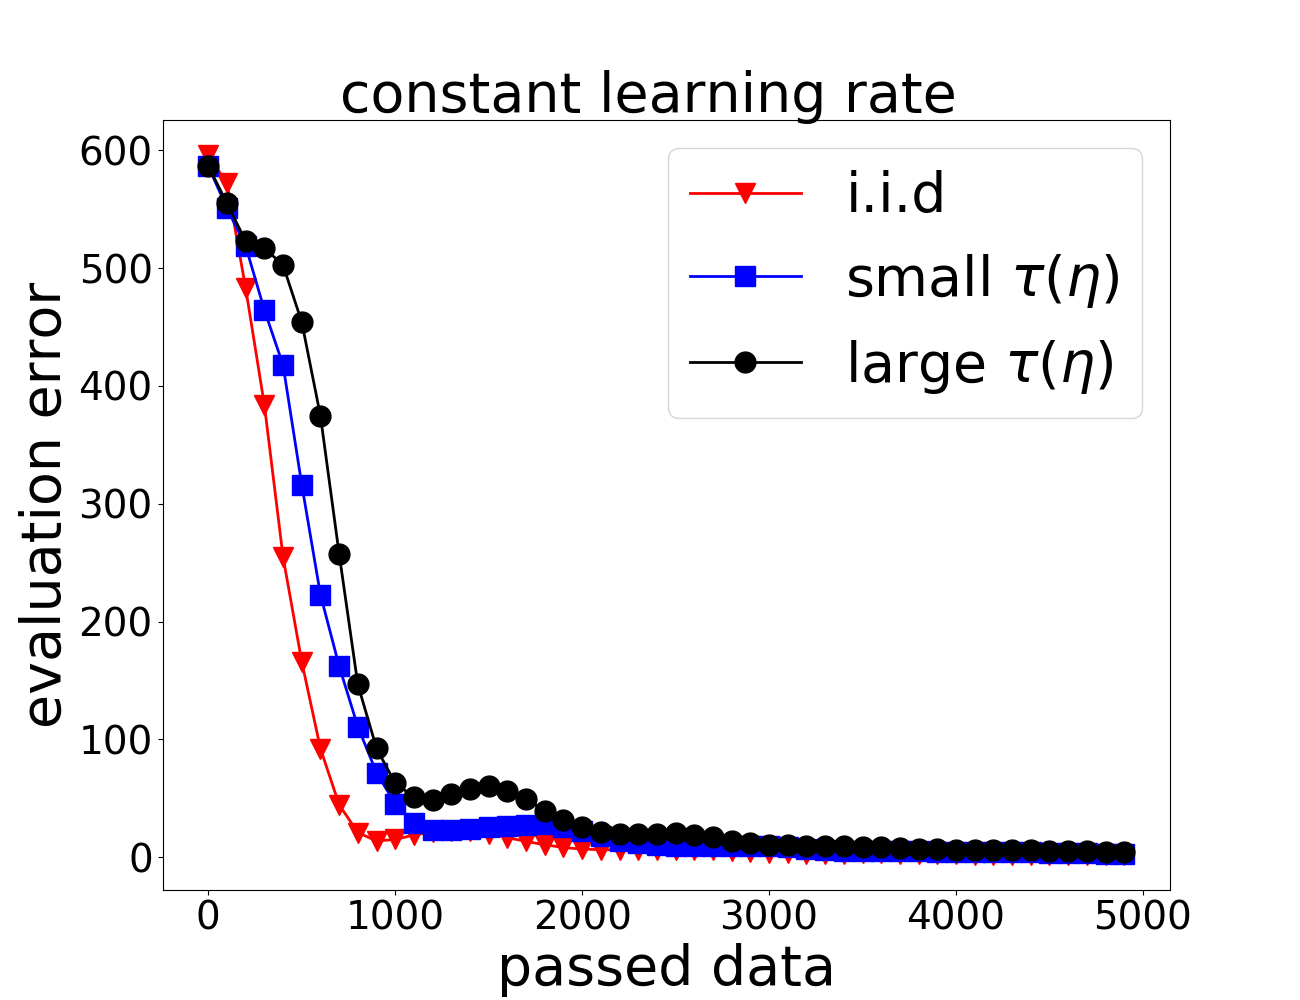
\includegraphics[width=1.5in,height=1.1in]{constant_learning_rate.png}}
		\subfigure[$ \alpha_t =\mathcal{O} (\frac{1}{\sqrt{t}}) $]{
			\label{figc}
			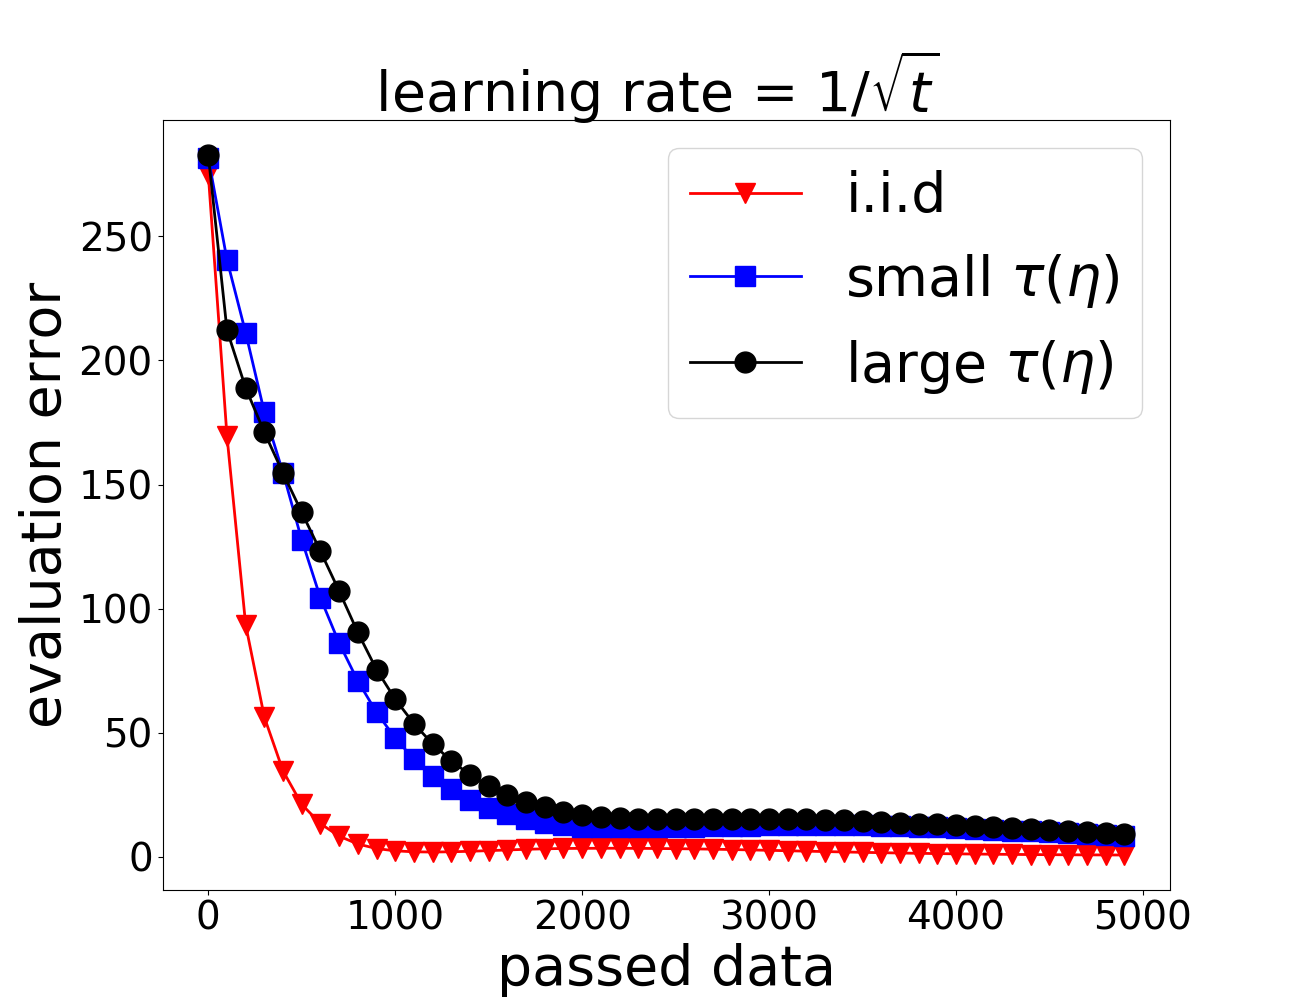
\includegraphics[width=1.5in,height=1.1in]{learning_rate_1st.png}} 
		\subfigure[$ \alpha_t = \mathcal{O} {(\frac{1}{t})}$ ]{
			\label{fige}
			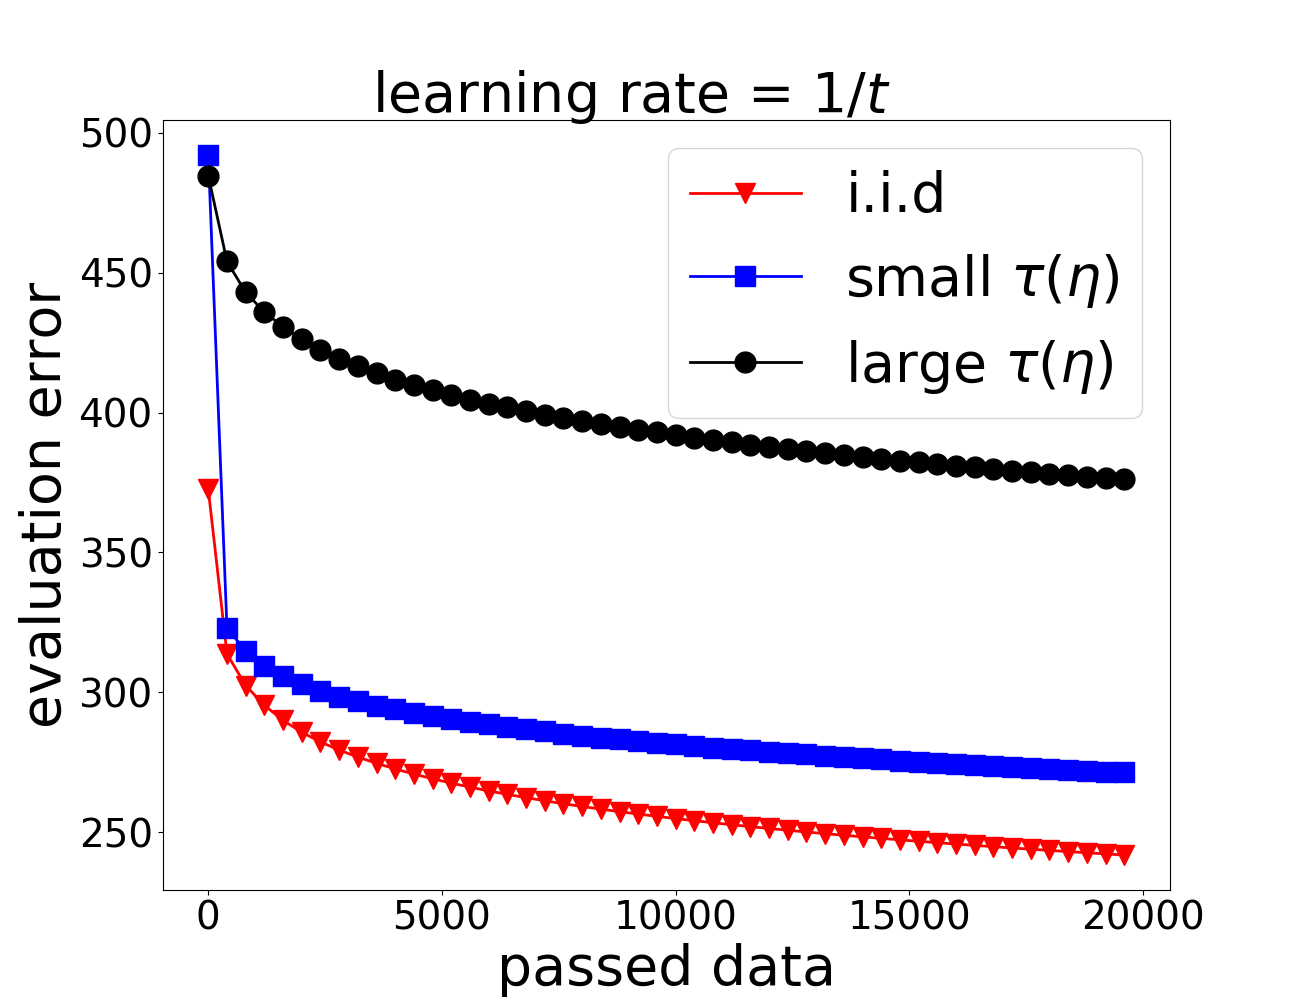
\includegraphics[width=1.5in,height=1.1in]{learning_rate_1t.png}}	
		\subfigure[$ \alpha_t  = c$ with trick  ]{
			\label{figb}
			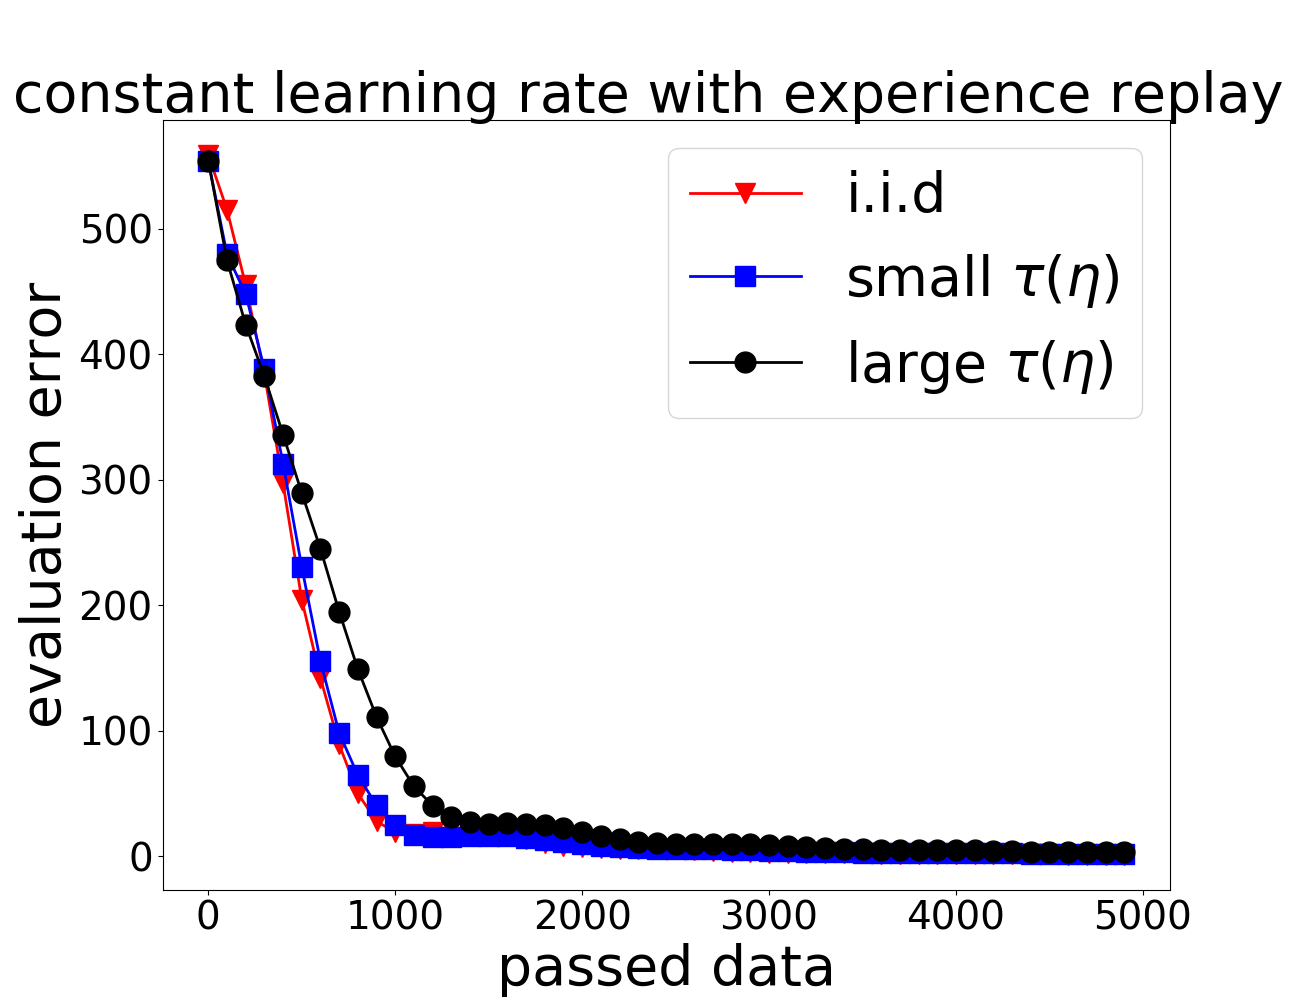
\includegraphics[width=1.5in,height=1.1in]{constant_learning_rate_with_experience_replay.png}}
		\label{Fig1}	
		\subfigure[$ \alpha_t =\mathcal{O}( \frac{1}{\sqrt{t}})$ with trick ]{
			\label{figd}
			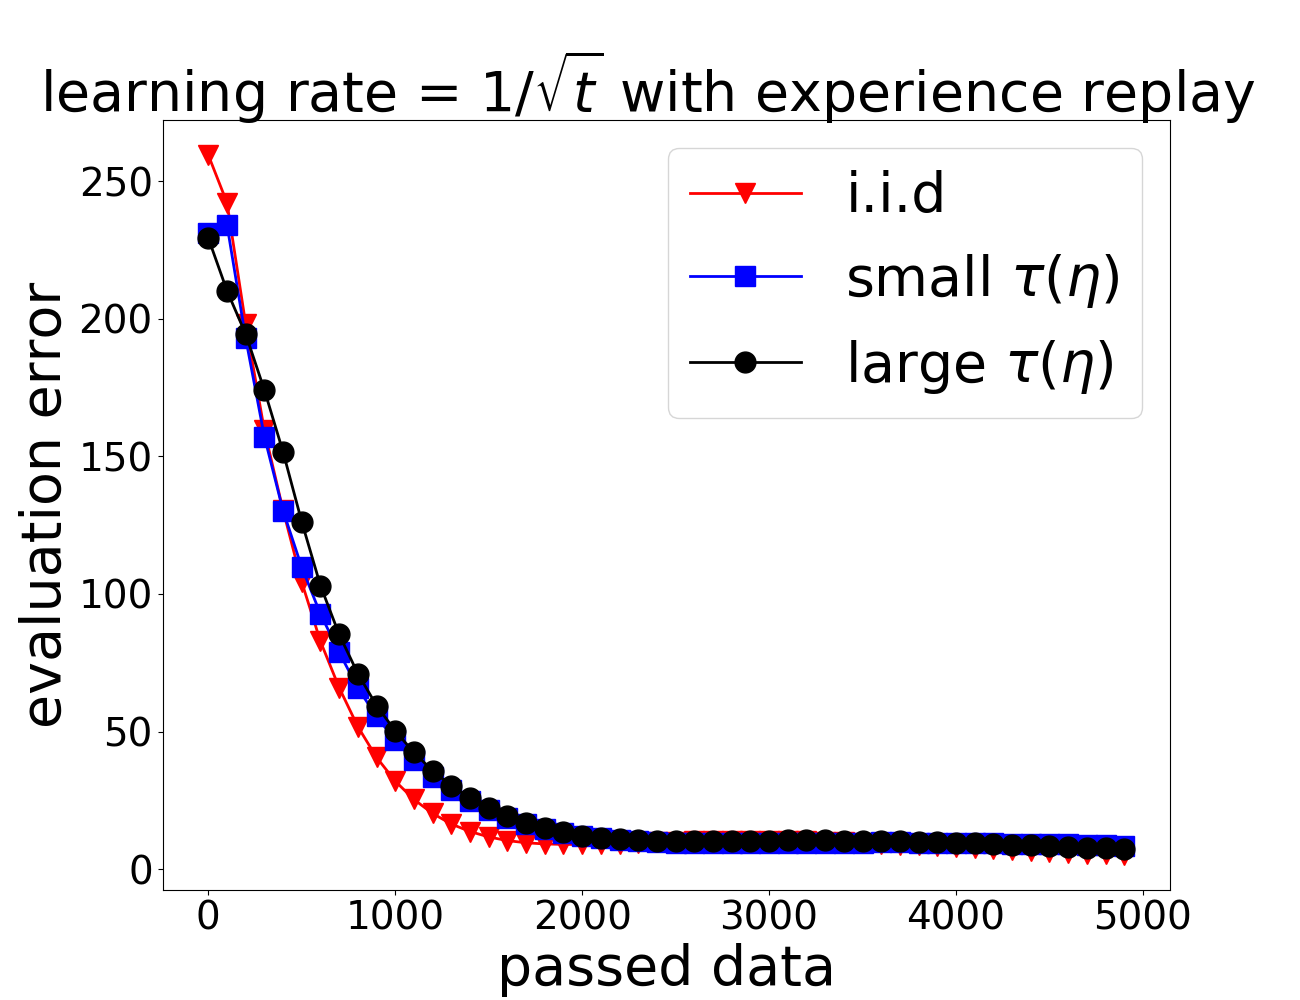
\includegraphics[width=1.5in,height=1.1in]{learning_rate_1st_with_experience_replay.png}}	
		\subfigure[$ \alpha_t =\mathcal{O} {(\frac{1}{t})}$ with trick  ]{
			\label{figf}
			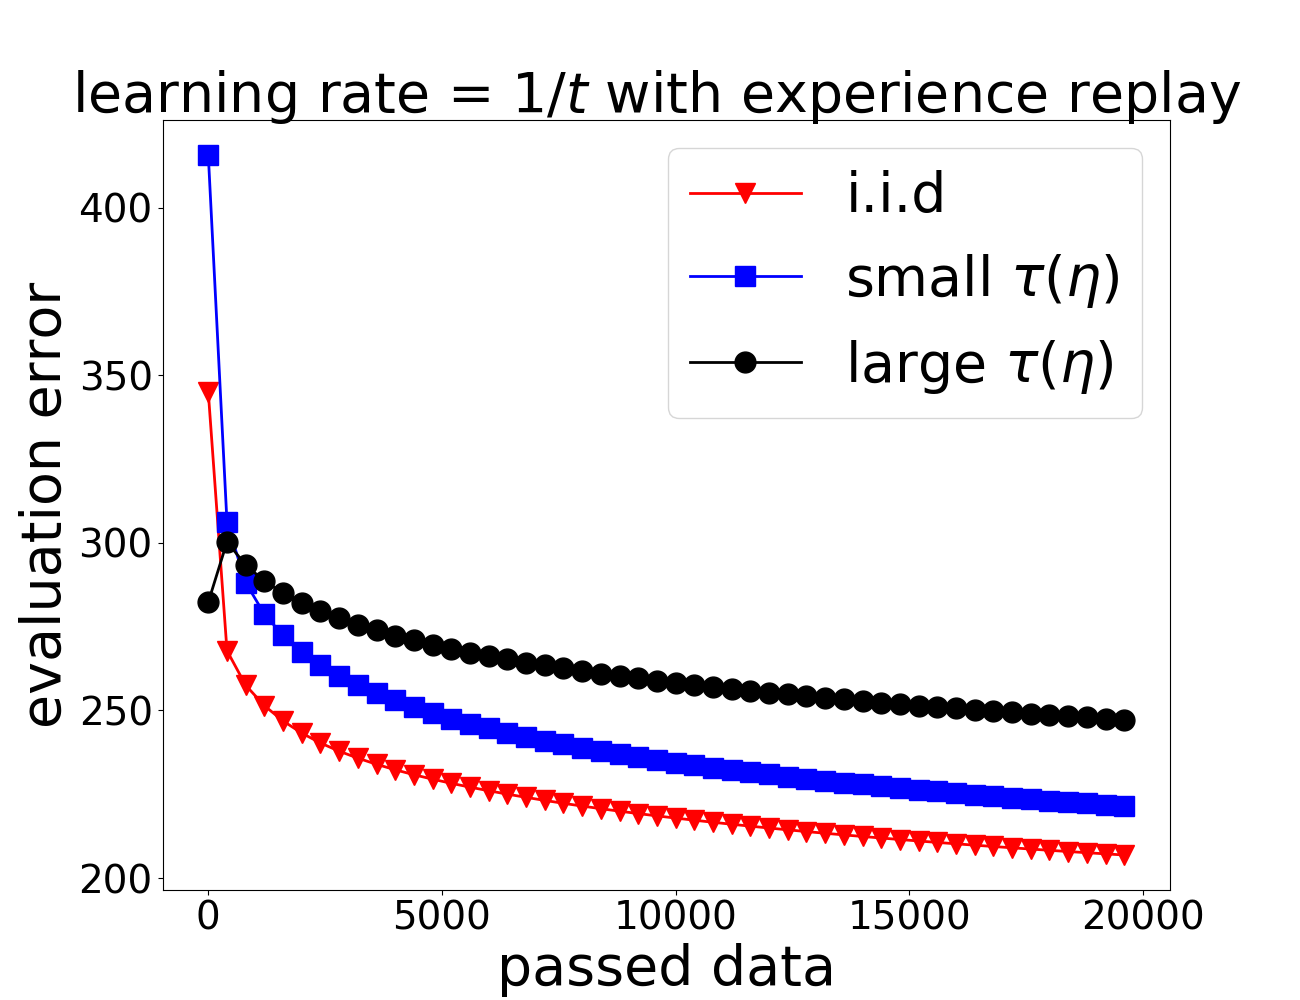
\includegraphics[width=1.5in,height=1.1in]{learning_rate_1t_with_experience_replay.png}}		
		\caption{Experimental Results  }		
	\end{figure*}	
	\section{Conclusion}
	In this paper, in the more realistic Markov setting, we proved the finite sample bound for the convex-concave saddle problems  in expectation and with high probability. Then, we obtain the finite sample bound for GTD algorithms both in on-policy and off-policy, considering that the GTD algorithms are specific convex-concave saddle point problems. Our finite sample bounds provide important theoretical guarantee to the GTD algorithms, and also insights to improve them, including how to setup the step size and we need to improve the mixing property of the data like experience replay. In the future, we will study the finite sample bounds for policy evaluation with nonlinear function approximation.


 
	
	
	
% Acknowledgements should go at the end, before appendices and references

%\acks{We would like to acknowledge support for this project
%from the National Science Foundation (NSF grant IIS-9988642)
%and the Multidisciplinary Research Program of the Department
%of Defense (MURI N00014-00-1-0637). }

% Manual newpage inserted to improve layout of sample file - not
% needed in general before appendices/bibliography.

\newpage

\appendix
\section*{Appendix A.}
\label{app:theorem}

% Note: in this sample, the section number is hard-coded in. Following
% proper LaTeX conventions, it should properly be coded as a reference:

%In this appendix we prove the following theorem from
%Section~\ref{sec:textree-generalization}:

In this appendix we prove the following theorem from
Section~6.2:

\noindent
{\bf Theorem} {\it Let $u,v,w$ be discrete variables such that $v, w$ do
not co-occur with $u$ (i.e., $u\neq0\;\Rightarrow \;v=w=0$ in a given
dataset $\dataset$). Let $N_{v0},N_{w0}$ be the number of data points for
which $v=0, w=0$ respectively, and let $I_{uv},I_{uw}$ be the
respective empirical mutual information values based on the sample
$\dataset$. Then
\[
	N_{v0} \;>\; N_{w0}\;\;\Rightarrow\;\;I_{uv} \;\leq\;I_{uw}
\]
with equality only if $u$ is identically 0.} \hfill\BlackBox

\noindent
{\bf Proof}. We use the notation:
\[
P_v(i) \;=\;\frac{N_v^i}{N},\;\;\;i \neq 0;\;\;\;
P_{v0}\;\equiv\;P_v(0)\; = \;1 - \sum_{i\neq 0}P_v(i).
\]
These values represent the (empirical) probabilities of $v$
taking value $i\neq 0$ and 0 respectively.  Entropies will be denoted
by $H$. We aim to show that $\fracpartial{I_{uv}}{P_{v0}} < 0$....\\

{\noindent \em Remainder omitted in this sample. See http://www.jmlr.org/papers/ for full paper.}


\vskip 0.2in
\bibliography{nips_2017}

\end{document}
